\section{Draft.} 

\subsection{Claim 13.}

\begin{claim}
  \label{claim:Tdeg} $d_{T} = ? $ \ctt{complete that lemma}. 
\end{claim}

\begin{proof}
Denote By $S_{e}$ the exceptional vertices in $\Gamma^{+}_{\square}$ which their degree restricted to $x$ is more than $\Delta^{1 \frac{1}{2} + \varepsilon}$ and we will say that any vertex which is not exceptional is normal.  

Let $T \subset V^{-}$ be the negative vertices which are connected to at least one normal vertex through an heavy edge i.e an edge which adjoins to at least $\delta\Delta - \Delta^{\frac{1}{2}}$ squares. 


\begin{equation*}
  \begin{split}
    & |S_{e}|\Delta^{1 \frac{1}{2}+ \varepsilon} \le \Delta^{2}|S_{e}|\frac{|S|}{n} +  \lambda \sqrt{|S||S_{e}|} \\ 
    & \left(  \Delta^{1 \frac{1}{2}+ \varepsilon} - \Delta^{2} \frac{|S|}{n}\right)|S_{e}| \le  \lambda \sqrt{|S||S_{e}|}\\
    & |S_{e}| \le \frac{\lambda^{2}}{\left(  \Delta^{1 \frac{1}{2}+ \varepsilon} - \Delta^{2} \frac{|S|}{n} \right)^{2}} |S| \le \frac{3}{4} |S|
  \end{split}
\end{equation*}


\begin{equation*}
  \begin{split}
    & \delta\Delta|T|\left( 1 - \frac{1}{\sqrt{\Delta}} \right) \le 2\Delta |T| \frac{|S|}{n} + \lambda_{\cup} \sqrt{|S||T|}\\ 
    & |T| \le \frac{\lambda_{\cup}^{2}}{ \left( \delta 2\Delta \left( 1 - \frac{1}{\sqrt{\Delta}} \right) -  \Delta \frac{|S|}{n} \right)^{2} } |S| \le \frac{1}{\Delta}|S|
  \end{split}
\end{equation*}


\begin{equation*}
  \begin{split}
    d_{T} = \frac{E(S_{n}, T)}{|T|} \ge \frac{|S_{n|}}{|T|} \ge   \left( 1 -  \frac{1}{\Delta} \right) \delta \Delta
  \end{split}
\end{equation*}

\end{proof}

\begin{equation*}
  \begin{split}
    (1- \frac{1}{2}\delta)\Delta^{2} \le \frac{3}{4}\left( 1 - \frac{1}{\sqrt{\Delta}}  \right)\Delta^{2} 
  \end{split}
\end{equation*}

Suppose that we have vertex $v_{-}$ which any of his positive neighbors contribute a row (col) with of poly-code with a small amount of noise (lets say below $\sqrt{\Delta}$). What could we say about the existence of polynomial that close to that manifold. We could think about that a linear number of rows has at most $\frac{1}{3}$ of zeros.  $ f\left( x,y \right)= \prod{ \left( x - a_{i} \right) \left(  y - b_{j} \right) } $


\ctt{ Seems like if $d_{T} \ge \theta \Delta^{2}$ then there is a little number of cols which are zero. Therefore we can think about some $f\left( x,y  \right) = \prod{ \left( y - a_{i} \right)   } g(x,y) $ such the degree of the first product is not so heigh and in addition if we write $f= l\left( x,y \right)g\left( x,y \right)$ then $l$ grantee that $f$ will agree on most to the zeros.  Now as the distance of the polynomial is relative large, we have that any term in $g$ after fixing $y$ is a low degree polynomial at $x$. Hence, it looks like ewe can only improve by adding the suit polynomial.}

\ctt{Notice that the product of two polynomial codes can be though as the polynomial in $2D$ in which the degree of each term is less than $2d$.} 

\begin{claim}
  \label{claim:poldu}
  Let $C_{0}$ be the $[\Delta,d, \Delta-d]$ polynomial code. Then any code word in $\left( C_{0}^{\perp} \otimes C_{0}^{\perp} \right)^{\perp}$ is a polynomial in $F[x,y]$ at degree at most $\Delta + d$
\end{claim}
\begin{proof}
Consider base element $ C_{0} \otimes \mathbb{F} $, denote it by $c = g_{i} \otimes e_{j}$. And notice that $c$ has representation in $F[x,y]$ of $\prod_{y^{\prime} \neq j}{\left( y - y^{\prime} \right) }g_{i}\left( x \right)$. By the fact that $g_{i}\left( x \right) \in C_{0} $ we have that degree of $c$ is at most $\Delta + \delta$. Hence any element in the subspace of $C_{0} \otimes \mathbb{F}$ is a polynomial at degree at most $\Delta + d$.   
\end{proof}

\ctt{ ToDo: Prove that $\prb{ P\left(x,y\right) = 0  } \le \frac{1}{\sqrt{RC}}$ where $x,y\sim [R]\times [C] \subset \mathbb{F}^{\Delta\times\Delta}$.  }

\begin{claim}
  \label{claim:lim}
  Any codeword in $\left( C_{0}^{\perp} \otimes C_{0}^{\perp} \right)^{\perp}$ at weight at most $\Delta^{1 \frac{1}{2}}$ is supported on at most $\Delta^{\frac{1}{2}} $ rows and columns.
\end{claim}
\begin{proof}
  Let $c$ be a codeword of the dual tensor and let $R (C)$ be the number of elements base at form $g_{i}\otimes e_{j} (e_{i} \otimes g_{j})$ on which $c$ has nonzero weight. Denote by $\delta_{0}$ the distance of the $C_{0}$. Now, denote by $\gamma$ the fraction number of interfere points between summed up vectors, and observe that by ~\cref{claim:poldu}, each of those point is a zero of polynomial at degree at most $\Delta + d$ over a subset $S \subset \mathbb{F}^{\Delta\times \Delta} $ at size $RC$.     

  Hence by Schwartz-Zippel lemma \cite{Schwartz} we have that $\gamma RC \le \left( d + \Delta \right)$. On the other hand, the number of weight of $c$ is at least: 
\begin{equation*}
    \begin{split}
      |c| \ge \left( R + C  \right) \delta_{0}\Delta - 2RC \cdot \gamma  \ge \left( R + C \right)\delta_{0}\Delta -2 \left( d + \Delta  \right)
    \end{split}
  \end{equation*}
  Combine the fact that $|c| \le \Delta^{1 \frac{1}{2}}$ we obtain that: 
  \begin{equation*}
    \begin{split}
      R + C \le 2\frac{d + \Delta}{\delta_{0} \Delta} + \frac{\Delta^{\frac{1}{2}}}{\delta_{0}}
    \end{split}
  \end{equation*}
\end{proof}
  
\begin{claim}
  Let $v_{-} \in T$ be a vertex adjoins to more than $\left( 1 - \frac{1}{\Delta} \right)\delta_{0}\Delta$ normal vertices via heavy edges. Then there exists $c \in C_{0} \otimes C_{0}$ supported on the local view of $v_{-}$ such that $|x + c| < |x|$. 
\end{claim}

\begin{proof}
  Noitce that any prumutation on the coordinate yield an euavlance code. Therefore if      

  \begin{center}
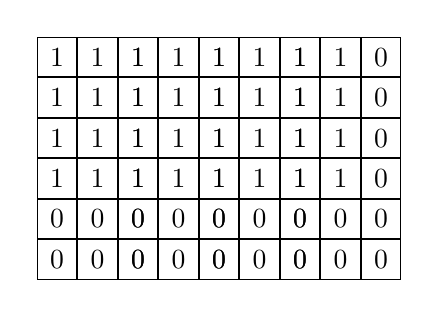
\begin{tikzpicture}
  %[every node/.style={draw=black}]
  \matrix[nodes={minimum size=5mm, draw=black}]
  {
    \node {1}; & \node{1}; & \node {1}; \node {1}; & \node{1}; & \node {1};\node {1}; & \node{1}; & \node {1}; \node {1}; & \node{1}; & \node {0};\\
    \node {1}; & \node{1}; & \node {1}; \node {1}; & \node{1}; & \node {1};\node {1}; & \node{1}; & \node {1}; \node {1}; & \node{1}; & \node {0};\\
    \node {1}; & \node{1}; & \node {1}; \node {1}; & \node{1}; & \node {1};\node {1}; & \node{1}; & \node {1}; \node {1}; & \node{1}; & \node {0};\\
    \node {1}; & \node{1}; & \node {1}; \node {1}; & \node{1}; & \node {1};\node {1}; & \node{1}; & \node {1}; \node {1}; & \node{1}; & \node {0};\\
    \node {0}; & \node{0}; & \node {0}; \node {0}; & \node{0}; & \node {0};\node {0}; & \node{0}; & \node {0}; \node {0}; & \node{0}; & \node {0};\\
    \node {0}; & \node{0}; & \node {0}; \node {0}; & \node{0}; & \node {0};\node {0}; & \node{0}; & \node {0}; \node {0}; & \node{0}; & \node {0};\\
  };
\end{tikzpicture}
\end{center}


\textbf{Warm-up.} Assume for the moment that any heavy edge contribute a low degree polynomial, and in addition, no interfere occurs. In other words, the rows and columns corresponds to heavy edges are polynomial at low degree and therefore the local view on $v$ is at distance at most $ \left( \Delta - C \right)\left( \Delta - R \right) $ from $C_{0}\otimes C_{0}$. That because one can obtains a valid codeword in $C_{0}\otimes C_{0})$ by setting values to the entries which don't supported by $R$ and $C$.  

That yield an upper bound on the difference $|x +c| - |x| \le  \left( \Delta -C \right) \left( \Delta -R \right) -  d_{T}\delta_{0}\Delta $. Note that the assumption that no interfere occurs is required for stating that we zeros at least $d_{T}\delta_{0}\Delta$ entries. Now, use the average inequality to obtain:   
\begin{equation*}
  \begin{split}
    \left( \Delta -C \right) \left( \Delta -R \right)  \le \left( \Delta - \frac{1}{2}\left( R+C \right)  \right)^{2}   = \left( \Delta - d_{T}/2 \right)^{2}
  \end{split}
\end{equation*}
Hence, any solution that satisfies the inequality $ \left( \Delta -d_{T}/2  \right)^{2} \le d_{T}\delta_{0}\Delta $ would grantee that $|x +c| < |x|$. Namely:
\begin{equation*}
  \begin{split}
   & d_{T} \in \left( - 2 \Delta \sqrt{\delta_{0} \left(\delta_{0} + 2\right)} + 2 \Delta \left(\delta_{0} + 1\right), 2 \Delta \sqrt{\delta_{0} \left(\delta_{0} + 2\right)} + 2 \Delta \left(\delta_{0} + 1\right)\right) \\
  \Rightarrow &  d_{T} \ge 2 \Delta + 2 \Delta \delta_{0} - 2 \sqrt{2} \Delta \sqrt{\delta_{0}} - \frac{\sqrt{2} \Delta \delta_{0}^{\frac{3}{2}}}{2} + O\left(\delta_{0}^{2}\right)
  \end{split}
\end{equation*}
And observe that if $\delta_{0} \ge \frac{1}{2}$ then $  2 \sqrt{2} \Delta \sqrt{\delta_{0}}  + \frac{\sqrt{2} \Delta \delta_{0}^{\frac{3}{2}}}{2} \ge 2\Delta + \Delta\delta_{0}$. Hence it's enough to require that: $d_{T} \ge \Delta \delta_{0}$. For picking $\delta_{0}$ slightly better and combining the fact that $d_{T} \ge \left( 1 - 1/\Delta \right)\delta_{0}\Delta$ we obtain correctness for the private case.  

%
%\begin{equation*}
%  \begin{split}
%    & \max \left( \Delta - C \right)\left( \Delta - R  \right) \\ 
%    & C + R \ge d_{T} \ge \left( 1 - \frac{1}{\Delta} \right)\delta_{0}\Delta
%  \end{split}
%\end{equation*}
%
%$\left( \Delta - C \right)\left( \Delta - R  \right) \le \left(1 - \left( 1 - \frac{1}{\Delta} \right)\delta_{0}/2  \right)^{2}\Delta^{2}$ 
%
%

\begin{equation*}
  \begin{split}
    d_{T} \in  \left\{\Delta \left(\delta_{0} + 2\right) - \sqrt{\Delta^{2} \left(\delta_{0} + 2\right)^{2} - 4 \Delta^{2} - 4 \Delta^{1.5}}, \Delta \left(\delta_{0} + 2\right) + \sqrt{\Delta^{2} \left(\delta_{0} + 2\right)^{2} - 4 \Delta^{2} - 4 \Delta^{1.5}}\right\}
  \end{split}
\end{equation*}

\begin{equation*}
  \begin{split}
    \left\{2 \Delta \left(\delta_{0} + 1\right) - 2 \sqrt{\Delta^{2} \left(\delta_{0} + 1\right)^{2} - \Delta^{2} - \Delta^{1.5}}, 2 \Delta \left(\delta_{0} + 1\right) + 2 \sqrt{\Delta^{2} \left(\delta_{0} + 1\right)^{2} - \Delta^{2} - \Delta^{1.5}}\right\}
  \end{split}
\end{equation*}
%The maximal point obtained when $C=R$ and therefore 

Denote by the number $R $ and $C$ the numbers of rows and columns with weight $\ge \phi \Delta$. We can set on $R\times C$ a codeword  
                        
  %By \cref{claim:Tdeg}  there exists at least one vertex $v_{-}$ 
                        
\end{proof}             

\subsection{Simplified Claim 13.} 
\newcommand{\Gtt}{\tilde{G}}
% \text{ if the row (col) } [uv] \text{ weight is } \Teta\left( \Delta \right) 
Denote by $\Gtt$ the graph obtained by $\Gtt  = \left\{ \left\{ u^{-}, v^{+} \right\}  \right\} $. By the assumption that $x$ is not a reducible we have that there exists $\gamma$ ( $ 1- \frac{1}{2}\delta$  )  such that the degree of any negative vertex in $\Gtt$ is less than $\gamma\Delta$. Denote by $S$ and $T$ the subsets of positive and the negative vertices on the support of $x$. By counting arguments we obtain that: 
\begin{equation*}
  \begin{split}
    |S| 2\Delta \ge E|_{\Gtt} \ge  |T| \Rightarrow \frac{|S|}{|T|} \ge \frac{\Delta}{2}
  \end{split}
\end{equation*}
We could also think on $S$ the normal vertices defined at \cite{leverrier2022quantum} (as been with positive degree in $\Gtt$ equivalence for been connected with heavy edge. On the other hand that quotient is also lower bound for the average degree of the negative vertices, Since $E_{\Gtt}(S,T)/|T| \ge |S|/|T| \ge \gamma/2$. For any random variable $X$ such that $X \le \Delta$ we have that: 

  \begin{equation*}
    \begin{split}
      & \prb{X\le x}x+\prb{X > x}\Delta\ge \expp{X}\Rightarrow \\ 
      & \prb{X \ge \frac{1}{2} \expp{X} } \ge \frac{\expp{X}}{2\Delta}
    \end{split}
  \end{equation*}

